\part{Modeling the afterglow of MMT170817}

%\begin{multicols}{2}
As insisted upon in the introduction, the GRB and afterglow counterparts of MMT170817 are \it{atypical} events. Nonetheless, the numerous observations of remnants and afterglows of transient electromagnetic events (such as supernovae and gamma ray bursts) indicate a common explanation of afterglows having timescales from days to years, such as that of MMT170817. Matter which is ejected during the previous phases of the phenomenon travels in the local external medium faster than the speed of sound. A shock thus forms at the interface of this ejecta with the interstellar medium. Interstellar material accumulates at this shock front, and its electrons are accelerated to an energized population and radiate through the synchrotron process in the magnetic field of the shock. As the material accumulates, the shock decelerates. As in Figure \ref{shock}, the \it{contact discontinuity} separates the ejecta and the energized swept-up interstellar material, which radiates from the \it{cooling zone}.

This is the overall vision of afterglows of events such as MMT170817. The exact nature and origin of the ejected matter, and the characteristics of the medium in which it evolves depends on the specific astrophysical phenomenon at hand. For example, in the case of core-collapse supernovae, the ejected matter is composed of the outer layers of the progenitor star. It is ejected with a quasi-spherical geometry and in form of a non- or mildly-relativistic shell. In the case of long GRBs, matter is ejected in the form of a jet (with a cone geometry) at ultra-relativistic velocities (Lorentz factors $\Gamma \gtrsim 100$).

\it{Which geometry, which dynamical structure, and which velocities were assumed by the ejectas of MMT170817?} We will confront afterglow data to different models in order to answer this question.

\fig{shock}{0.7}{Cut across the shock front, showing the ejected matter on the source side of the contact discontinuity, and the interstellar material accumulating at the forward shock front. Synchrotron radiation from the shock-accelerated electrons constitute the afterglow. The shocked ejecta (behind the \it{reverse shock}, red shaded region) also emits radiation, which we do not consider for this work, see Section \ref{modelization} for details.}{Schematic cut across the shock front}
\section{The physics of afterglows: deceleration dynamics, radiation and astronomical observables}

In this section, we will review the physics which will take part in the modeling of the afterglow of MMT170817. We will successively describe the deceleration of the remnant expanding in the interstellar medium, the synchrotron radiation of the shock-accelerated electrons, and derive the electromagnetic signals which arise from this radiation.

\subsection{Relativistic deceleration}
\label{dynamic}
We now describe the dynamics of the deceleration of the remnant in the ISM. We will consider for this work two different structures for the matter ejection. First, a \it{mono-kinetic ejecta} in which the ejection occurred at a single speed altogether. This model applies to cases where the ejection occurs on time scales much smaller than the time-variability time-scale of the ejecting engine. Secondly, a \it{radially stratified ejection}, where matter is ejected with a differential of speeds. This can correspond to a long and time-varying activity of the central engine\footnote{The dynamical time scale of the merged system --~that of the establishment of a accretion disk for example~-- is on the order of the period of a Keplerian orbit close to the final compact object, i.e $\sim$~1~ms. Thus, a long activity of the central engine is in our case one longer than about this time scale.}.

Let $r$ designate the radial coordinate of the shock front, counted in the exterior laboratory frame from the central engine out, and $\Gamma(r)$ the Lorentz factor of the shock once it has reached position $r$. We also introduce the velocity of the shock front $v(r) = \beta(r)c$.

\bf{Mono-kinetic ejection.} In this case, the matter is ejected with initial energy $E_0$ and a single Lorentz factor $\Gamma_0$. By plowing through the ISM, the shock sweeps up interstellar material and decelerates. The exact general self-similar solution of these dynamics is given in \citet{59}, but we will follow a simpler approach.

By denoting $M_{\rm{ej}}$ the mass of the ejected matter, $m(r)$ the accumulated mass swept up by the shock, conservation of energy implies that the initial total energy $\Gamma_0 M_{\rm{ej}} c^2 + m(r) c^2$ is distributed in the energy of the ejected mass $\Gamma(r) M_{\rm{ej}} c^2$ and the internal energy of the energized swept up mass $\Gamma(r)^2 m(r) c^2$. Thus:

\begin{equation}\Gamma(r)^2 m(r) c^2 + \Gamma(r) M_{\rm{ej}} c^2 = \Gamma_0 M_{\rm{ej}} c^2 + m(r)c^2 \end{equation}

Details on the $\Gamma^2 m c ^2$ form for the internal energy of the swept-up mass can be found in \it{Appendix A}. Grossly it is understood by writing the co-moving internal energy as $\Gamma m c^2$, and the boost to the lab frame introduces an additional $\Gamma$ factor.

In our case, the neutron star binary has long left the environment where the last of the two neutron-star-forming supernovae occurred, thus no massive-star wind outflow is present in the outskirts of the merger site, and we will consider for our purposes a homogeneous medium with number density $n$.

Suppose that the mass $M_{\rm{ej}}$ was ejected into a solid angle $\Omega$ by the central source, for instance in the form of a cone. Then if we neglect any lateral expansion of the ejected matter, the swept-up mass at radius $r$ will be\footnote{In all generality, we should consider the average mass per particle in the local exterior environment $\mu m_P$ instead of $m_P$. This would simply amount to changing $n$ into $\mu n$ for the rest of the calculation.}:

\begin{equation}m(r)~=~\Omega\int_0^r dr' r' ^ 2 n m_P\end{equation}

A hydrodynamic lateral expansion would occur at the speed of sound, thus it is correct to neglect any such expansion as long as the ejecta assumes relativistic speeds.

We introduce the dimensionless mass parameter $\eta(r) \equiv \frac{m(r)}{M_{\rm{ej}}/\Gamma_0}$. It writes:


\begin{align}
\eta(r) &= \frac{\Omega \int_0^r dr' r' ^ 2 n m_P}{M_{\rm{ej}}/\Gamma_0}  \\
 &= \frac{\Omega r ^ 3}{3 M_{\rm{ej}}/\Gamma_0} n m_P \\
 &= \frac{\Omega r ^ 3 n m_P }{3 E_0 / \Gamma_0^2 c^2}\\
 &= \left( \frac{r}{R_{\rm{dec}}} \right)^3
\end{align}

where we identify the \it{deceleration radius}, $R_{\rm{dec}}$, such that:

\begin{align}
    R_{\rm{dec}}^3 &= \frac{3 E_0}{\Omega n m_P \Gamma_0^2 c^2} \\
                   &= \frac{3 E_\rm{iso}}{4\pi n m_P \Gamma_0^2 c^2}
\end{align}

where $E_\rm{iso}$ is the isotropic-equivalent energy of the outflow.

Finally, the solution for $\Gamma(r)$ is easily found to be:

\begin{equation}\Gamma(r) = \Gamma_0 \frac{-1 + \sqrt{1 + 4\eta(r) + \frac{4\eta(r) ^ 2}{\Gamma_0^2}}}{2 \eta(r)}\end{equation}

\bf{Phases of deceleration.} We observe three phases in the deceleration of the shock front:

\begin{enumerate}
	\item For $\mu(r) \ll 1/4$, i.e $r \ll R_{\rm{dec}}$, in the \it{coasting phase}, no deceleration occurs:

	\cen{\Gamma(r) \simeq \Gamma_0}

    Thus, no deceleration occurs before a mass $M_{\rm{ej}}/\Gamma_0$ is swept-up.

	\item For $1/4 \ll \mu(r) \ll \Gamma_0 ^ 2$, i.e $R_{\rm{dec}} \ll r \ll \Gamma_0^{2/3} R_{\rm{dec}} \equiv R_{\rm{N}}$ (\it{Newtonian radius}), the front is in a \it{relativistic deceleration phase}, during which the swept-up mass progressively reaches $\Gamma_0 M_{\rm{ej}}$:

	\cen{\Gamma(r) \simeq \frac{\Gamma_0}{\sqrt{\mu(r)}} = \Gamma_0 \left(\frac{r}{R_{\rm{dec}}} \right) ^ {-3/2}}

    The slope --3/2 found for this regime is identical to that of \citet{59}.

	\item For $\Gamma_0^2 \ll \mu(r)$, i.e $ R_{\rm{N}} \ll r$:

	\cen{\Gamma(r) \simeq 1}

	and

	\cen{v(r) \simeq c  \left( \frac{r}{R_{\rm{N}}} \right) ^ {-3/2} \simeq \left( \frac{3 E_\rm{iso}}{4\pi n m_P}\right)^{1/3}r^{-3/2}}

	This is the \it{Newtonian phase}, and we see that deceleration to non-relativistic velocities requires the sweeping up of a mass on the order of $\Gamma_0 M_{\rm{ej}}$. This regime of the dynamics is the same as the Sedov solution \citep{60}, which is valid for non-relativistic cases.
\end{enumerate}

\bf{Radially stratified structure.} In this case, we suppose that the matter was ejected with an inhomogeneous distribution of velocities: some components were ejected with larger energies than others, as in a continuous and decreasing activity of the central engine. We parametrize this distribution giving a cumulative distribution $E( > \Gamma)$ of energies. It is such that at ejection, the total energy of the matter having a Lorentz factor larger than a given $\Gamma$ is $E( > \Gamma)$. Note that here, we always consider spherical ejections and thus identify any quantity with its isotropic equivalent.

After the ejection, the higher-velocity component of the ejecta will form the shock front, while the rest of the ejecta lags behind. The front shock decelerating in the ISM, the slower components will catch up to the front shock. This way, the catching-up matter will slow the deceleration down, until the slowest component has caught up. Then, the dynamics are the same as a mono-kinetic ejection starting from the slowest initial velocity.

How to write energy conservation in this model? We will simplify the problem and neglect the time it takes for matter to catch-up to the shock. In this case, if the front shock has reached a Lorentz factor $\Gamma$ (at $r$), it means that all the energy which was initially available to the ejected matter with Lorentz factors above $\Gamma$ has already caught-up and been injected into the shock. Moreover the energy injected to the shock is held in internal energy by the swept-up material at the shock, as in the mono-kinetic ejection case. Thus, we have:

\begin{equation} \Gamma(r)^2 m(r) c ^ 2 = E( > \Gamma(r)) + m(r) c ^ 2\end{equation}

Notice that this is an implicit equation on $\Gamma(r)$. In addition, we do not consider here an initial bulk mass which would have an initial energy of $\Gamma_0 M c^2$. Considering an additional bulk mass in this process would simply amount to a discontinuous function $ E( > \Gamma)$.

In the case of a homogeneous medium, this reduces to:

\begin{equation}\frac{4\pi}{3}r^3 n m_P c^2(\Gamma(r)^2 - 1) = E( > \Gamma) \end{equation}


Alternatively, we parametrize the distribution in terms of the \it{relativistic 4-velocity} $u = \Gamma \beta$. This allows us to consider non-relativistic velocities ($u \sim 0$) as well as ultra-relativistic cases ($u \gg 1$), as the nature of the outflow responsible for the afterglow of MMT170817 is quite uncertain.

If the total initial energy is $E_0$ and the largest (resp. smallest) velocity in the ejecta is $u_M$ (resp. $u_m$), then the energy distribution function can be written as:

\begin{equation} E( > u) = E_0\, g(u) \end{equation}

where $g$ is a function equal to 1 for $u < u_m$, to 0 for $u_M < u$, and decreases between $u_m$ and $u_M$.

A simple functional form for $g$ which meets these requirements is a power-law with some positive index $\alpha$ containing all the unknown physics of the ejection event, such as:

\begin{equation}
    g(u) = \left \{ \begin{array}{cl}
    1 & \text{if } u < u_m \\
    \frac{u ^ {-\alpha} - u_M^{-\alpha}}{u_m ^ {-\alpha} - u_M ^ {-\alpha}} & \text{if } u_m < u < u_M \\
    0 & \text{if } u_M < u
\end{array}
    \end{equation}

In this case, the final deceleration dynamics equation is (note that $\Gamma^2 - 1 = (\Gamma\beta)^2$):

\begin{equation}\frac{4\pi r^3 n m_P c^2u(r)^2}{3 E_0} = \frac{u(r) ^ {-\alpha} - u_M^{-\alpha}}{u_m ^ {-\alpha} - u_M ^ {-\alpha}} \end{equation}

In this case, solving for $\Gamma(r)$ (or equivalently $u(r)$) is not analytical, and we will find $\Gamma(r)$ with help of numerical solving, by the bisection method in our case. For our purposes, we fix the value of $\alpha$ to the fiducial value of 5 \citep{13}. Having explored other values for $\alpha$ between $2$ and $7$, we concluded that the qualitative form of the results were unchanged.

\subsection{Synchrotron radiation and self-absorption}
We now turn to the radiation emerging from the shocked matter, which constitutes the afterglow emission. From now on, we will denote with primes $\p$ the value of quantities measured in a frame co-moving with the shocked emitted matter, and without primes those measured in the laboratory (exterior) frame.

\bf{Shock conditions on number density and specific internal energy. }What are the conditions at the shock front, where electrons are accelerated and radiate? They are given by the Rankine-Hugoniot \citep[e.g][chap. 15]{39} relations. In strong shocks, the shocked matter's internal energy is much larger than its rest mass energy. We thus consider the conditions for ultra-relativistic matter (with an adiabatic index of $\gamma = 4/3$). Then, the shock-frame number density $n\p$ and ratio of internal energy to mass energy $\epsilon\p$ are:

\begin{equation}n\p = (4 \Gamma + 3) n\end{equation}

and

\begin{equation}\label{ep}
    \epsilon\p = (\Gamma - 1)
\end{equation}

\bf{Electron population and magnetic field. }The physical process we consider for radiation is synchrotron radiation. The energy deposited by the shock contributes to the two factors of synchrotron radiation: a magnetic field and a population of relativistic electrons.

The microphysics of the emergence of magnetic fields and energized populations of electrons in astrophysical shocks are an area of intense research. From our standpoint, we are concerned only with the strength of the field, and will consider that a free microphysical \it{redistribution} parameter $\epsilon_B$ relates the field magnitude to the shock-frame energy density. More explicitly, we define $\epsilon_B$ such that in the shock frame, a fraction $\epsilon_B$ of the internal energy density is in the form of magnetic energy from the entangled magnetic field. Thus:

\begin{equation}\frac{B\p^2}{8\pi} = \epsilon_B n\p \epsilon\p m_P c^2\end{equation}

Likewise, we will consider that in the electron population, the Lorentz factor has a simple probability density $\mathcal{N}(\gamma)$: it is a power law of index $p > 2$ in the Lorentz factor space as of some minimal Lorentz factor $\Gamma_m$, as in the case of populations energized by high-energy astrophysical processes such as Fermi acceleration\footnote{Any acceleration process having a maximum energy, we could also have introduced a maximum Lorentz factor of the electron population. This would have slightly complicated this derivation.}, that is:

\begin{equation}
    \mathcal{N}(\gamma) \propto \left \{ \begin{array}{cl}
    0 & \text{if } \gamma < \gamma_m\\
    \gamma^{-p} & \text{if } \gamma_m < \gamma
\end{array}
\end{equation}

Note that the energy contained in the electron population is \it{not directional}. On the contrary to the exterior kinetic energy of the shock (encompassed in $\Gamma(r)$), this electron energy distribution arises from an isotropic momentum distribution in the local frame, and thus may be regarded as internal energy.

We introduce yet another microphysical redistribution parameter $\epsilon_e$, which relates the proportion of the local internal energy which is carried by the energized electrons. By requiring that the electrons carry a fraction $\epsilon_e$ of the total internal energy, we write:

\begin{equation}\int_{\gamma_m}^\infty d\gamma \mathcal{N}(\gamma)\gamma m_e c^2 = \epsilon_e \epsilon\p m_P c^2\end{equation}

Also, normalization of the probability density writes:

\begin{equation}\int_{\gamma_m}^\infty d\gamma \mathcal{N}(\gamma) = 1 \end{equation}

With these two, one obtains:

\begin{equation}\label{w}
    \gamma_m= \epsilon_e \frac{m_P}{m_e}\frac{p - 2}{p - 1} (\Gamma - 1)
\end{equation}

and finally we have:

\begin{equation}\label{N}
    \mathcal{N}(\gamma) = \left\{ \begin{array}{cl}
                                    0 & \text{for }\gamma < \gamma_m\\
                                    \frac{p-1}{\gamma_m}\left(\frac{\gamma}{\gamma_m}\right)^{-p} & \text{for }\gamma_m < \gamma
                                    \end{array}\right.
\end{equation}

As of now, we will fix the value of $\epsilon_e$ to the fiducial value of 0.1. This value is supported by the fitting of synchrotron models such as ours to GRB afterglows \citep[see e.g][]{41}.\\

\bf{The synchrotron spectrum of a power-law population of electrons. }It can be shown  \citep[see e.g][sec. 6]{55} that the source-frame synchrotron spectral power emitted by a single electron of Lorentz factor $\gamma_e$ in a magnetic field $B\p$ varies as $\nu\p^{1/3}$ until a maximum frequency:

\begin{equation}\label{q}
    \nu_s\p(\gamma_e) = \gamma_e^2 \frac{eB\p}{2\pi m_e c}
\end{equation}

and then decreases exponentially. The maximum spectral power (units of erg/s/Hz) is:

\begin{equation}\label{pmax}
    P_\rm{max}\p = \frac{m_e c^2 \sigma_T}{3e}B\p
\end{equation}

where $\sigma_T$ is Thomson cross-section.

It follows that the total power emitted by the electron (units of erg/s) is approximately:

\begin{align}
    P\p &\simeq \int_0^{\nu_s\p(\gamma_e)} d\nu\p P_\rm{max}\p \left(\frac{\nu\p}{\nu_s\p(\gamma_e)}\right)^{1/3} \\
        &\simeq P_\rm{max}\p \nu_s\p(\gamma_e)
\end{align}

Thus the time scale for energy loss by synchrotron radiation is:

\begin{align}
    t_r\p &= \frac{\gamma_e m_e c^2}{P\p} \\
          &= \frac{6\pi m_e c}{\sigma_T \gamma_e B\p^2}
\end{align}

How does this compare to the time scale for adiabatic cooling due to the expansion of the shell?

The exterior frame expansion time scale (the \it{dynamical} time-scale) is $t_d = \frac{v}{R}$, needed for the remnant to double its radius. In the shock-frame this is $t_d\p = \frac{v}{\Gamma R}$.

We denote by $\gamma_c$ the Lorentz factor of an electron which cools by synchrotron radiation in a dynamical time-scale, i.e $t_r\p = t_d\p$. In other words:

\begin{equation} \gamma_c = \frac{6 \pi m_e c}{\sigma_T B\p^2 t_d\p}\end{equation}

It follows that for an electron with $\gamma_e > \gamma_c$, the cooling by synchrotron radiation occurs on a time-scale smaller than by adiabatic cooling. We call this state \it{fast cooling}. On the other hand, a population of electrons with $\gamma_e < \gamma_c$ cools by adiabatic expansion more efficiently than by radiation. We call this \it{slow cooling}.

Furthermore, we introduce the synchrotron characteristic frequencies of the electron population $\nu_m\p$ and $\nu_c\p$ as the frequency of peak emission from electrons with Lorentz factors $\gamma_m$ and $\gamma_c$:

\begin{align}\label{freqs}
    \nu_c\p &= \nu_s\p(\gamma_c) \\
    \nu_m\p &= \nu_s\p(\gamma_m)
\end{align}

For a fast cooling electron, the total energy goes as $E \propto \gamma_e$, whereas the radiated power is as $P' \propto \gamma_e^2$. Thus as the electron cools from $\gamma_e$ to $\gamma_c$, the bulk of the radiation is emitted on the $[\nu_c', \nu_e']$ portion of the spectrum, where the spectral power is $\propto \nu\p^{-1/2}$.

The overall power spectrum for a single electron is thus composed of three segments: a power law as $\nu\p^{1/3}$ for $\nu\p < \nu_c\p$, a power law as $\nu\p^{-1/2}$ for $\nu\p_c < \nu\p < \nu_s\p(\gamma_e)$, and an exponential cut-off for larger frequencies. The maximum spectral power is $P_\rm{max}\p$, attained at $\nu_c\p$.

Coming back to the entire population of the electrons in the shock, we determine the total emission spectrum by integrating on the Lorentz factor distribution $\mathcal{N}$ as in Eq.~\ref{N}. For this, two cases can arise:

\begin{enumerate}
    \item $\gamma_m < \gamma_c$: thus the bulk of the population has $\gamma_e < \gamma_c$ and is in slow cooling. Then, the average power spectrum per electron is\footnote{Here, we neglect a numerical factor close to unity arising from the exact integration on the population.}:

    \begin{equation}
        \label{s1}
        P\p = P_{\rm{max}}\p \times \left\{ \begin{array}{cl}
                         (\nu\p/\nu\p_m)^{1/3} & \text{for } \nu\p < \nu\p_m \\
                         (\nu\p/\nu\p_m)^{-(p-1)/2} & \text{for }  \nu\p_m < \nu\p < \nu\p_c \\
                         (\nu\p_c/\nu\p_m)^{-(p-1)/2}(\nu\p/\nu\p_c)^{-p/2} & \text{for }  \nu\p_c < \nu\p
                         \end{array}\right.
    \end{equation}

    \item $\gamma_c < \gamma_m$: thus all of the electrons are in fast cooling. Then, the average power spectrum per electron is:

    \begin{equation}
        \label{s2}
        P\p = P_{\rm{max}}\p \times \left\{ \begin{array}{cl}
            (\nu\p/\nu\p_c)^{1/3} & \text{for }  \nu\p < \nu\p_c \\
            (\nu\p/\nu\p_c)^{-1/2} & \text{for }  \nu\p_c < \nu\p < \nu\p_m \\
            (\nu\p_m/\nu\p_c)^{-1/2}(\nu\p/\nu\p_m)^{-p/2} & \text{for }  \nu\p_m < \nu\p
                         \end{array}\right.
    \end{equation}
\end{enumerate}

\bf{Synchrotron absorption and inverse-Compton diffusion.} In addition, we may consider the absorption of the synchrotron radiation from the electron population itself, as well as the inverse-Compton diffusion of the synchrotron radiation. Results show  \citep[see e.g][]{1} that these effects are negligible in our case of radio synchrotron emission.

\subsection{Derivation of the astronomical observable: flux density}

Given a rest-frame emission spectrum for the matter in the expanding shock and a velocity of the shock, what flux will a distant observer measure? Suppose that at exterior time $t = 0$, the matter is ejected, and that the shell has reached a radius of $R$ and Lorentz factor $\Gamma$ by time $t$. Suppose a chunk of matter in the shock front emits some light with frequency $\nu\p$ in its rest frame. We must discuss the arrival time and frequency of the light to the observer.

\fig{schema}{0.6}{The geometry of the remnant. A spherical shell-like shock front (or a part of a sphere) is expanding at speed $\beta(t)$, while the population of energized electrons radiates in its own reference frame according to an emissivity $j\p$.}{The geometry of the remnant}

\bf{Simple discussion: matter moving towards the observer. }Suppose that the emitter is moving towards the observer, like the red dot in Figure \ref{schema}. Then the observed frequency at the time of arrival of the emitted light will simply be $\nu = \frac{\nu\p}{\Gamma(1 - \beta)}$ by relativistic Doppler shifting\footnote{There are many conventions for the expression of the Doppler factor and the sign of $\beta$. Noticing that $\Gamma(1 + \beta) = \frac{1}{\Gamma(1 - \beta)}$, we might have as well written $\nu = \Gamma (1 + \beta) \nu\p$.}. Note that in the case of an ultra-relativistic outflow (for a GRB for example, where $\Gamma \gtrsim 100$), we will have $\nu \simeq 2 \Gamma \nu\p$, inducing an extremely important effect. Here, $\Gamma$ and $\beta$ here must be considered at the time of emission $t$ of the light of course.

Let $\tobs$ denote the time of arrival to the distant observer of the light emitted at $t$. After emission, the light travels the distance $D - R$ before arrival. Thus, $\tobs = t + \frac{D - R}{c}$, where $D/c$ here is nothing else than the 120~Myr the first emitted light took to reach us. If we count time from the observer-frame beginning of the event, we can drop this delay, and thus write:

\begin{equation}\label{tobs}
    \tobs = t - R/c
\end{equation}

The dynamics are of course counted starting from the time of ejection. Thus we will set $t = \tobs =0$ and $R = 0$ at the time of ejection\footnote{The measured light curves from the afterglow are given with time counted from the GW-inferred time of merger. The afterglow time-scale being on the order of days, neglecting the delay between the merger time ($t = 0$ of the observed light curves) and the time of ejection ($t = 0$ of our model) is an acceptable approximation.}. Let us introduce the shock-frame time coordinate $t\p$, such that $dt\p = dt/\Gamma(t)$ and $t\p = 0$ at ejection.

What flux will be received from this chunk of emitting matter? We introduce the rest-frame emissivity $j\p$ of the matter (units of erg/s/cm\sp{3}/Hz). The power emitted isotropically in all rest-frame directions at shock-frame time $t\p$ by a volume $dV\p$ of this matter in the rest-frame frequency interval $d\nu\p$ around $\nu\p$ is $j\p(\nu\p, t\p)dV\p d\nu\p$. Through Lorentz transformations, it can be shown that $j/\nu^2$ is conserved \citep[see e.g][sec. 4]{55}.

It thus follows that the received spectral flux density (in units of ergs/s/cm\sp{2}/Hz) at observer time $\tobs$ and frequency $\nu$ will be:

\begin{equation}dF(\nu, \tobs) = \frac{1}{4\pi D^2} \frac{j\p(\nu \Gamma(t)(1 - \beta(t)), t\p)}{(\Gamma(t)(1 - \beta(t)))^2}dV\end{equation}

where $t$ and $t\p$ are simply the source-frame and shock-frame time coordinates of the event of the emission of the light which was received at observer time $\tobs$. Of course, since the dynamics of the shell are followed according to $t$, we will express $j\p$ as a function of $t$ later.

\bf{General discussion: flux from an extended remnant.} Let us now consider a chunk of matter moving with an angle $\theta$ with respect to the line of sight (like the blue dot on Figure \ref{schema}). We introduce the general form of the Doppler factor:

\begin{equation}\label{doppler}
\mathcal{D}(\theta) = \frac{1}{\Gamma(1 - \beta \cos \theta)}
\end{equation}

Then the Doppler shifting reads more generally $\nu = \mathcal{D}(\theta)\nu\p$, and the distance to travel for the light from emission to reception is $D - R \cos \theta$, thus the time of arrival is:

\begin{equation}
\tobs = t - R \cos \theta / c
\end{equation}

Notice that in this case, for a same arrival time, the time of emission is dependent on $\theta$ in such a way that at one given instant, the observer is receiving light emitted by the shell at earlier times (and thus different $\beta$ and $j\p$) for larger angles from the line of sight.

Thus, by neglecting absorption and diffusion of radiation from the remnant, we write the total flux measured at time $T$ as:


\begin{equation}\label{in}
    F(\nu, T) = \frac{1}{4\pi D ^ 2}\int_0^{\infty} dt \int_0^\infty dr \int \int_{\Omega_E} d\theta d\phi r^2 \sin \theta \,\mathcal{D}(\theta, t)^2 \left[ j\p\left(\frac{\nu}{\mathcal{D}(\theta, t)}, r, t\right) \delta\left(T - t + \frac{r\cos\theta}{c}\right) \right]
\end{equation}


where $\mathcal{D}(\theta, t) = \frac{1}{\Gamma(t)(1 - \beta(t) \cos \theta)}$ is the time-dependent Doppler factor of the matter of which the radiation will be received at $T$, and $\Omega_E$ is the total solid angle occupied by the remnant. This equation takes into account the delay on light arrival time (through the $\delta$ function), the Doppler frequency shifting (through the evaluation of $j\p$ at $\nu/\mathcal{D}$) and the relativistic beaming of radiation (through the integration of $j\p/\mathcal{D}^2$).

For a spherical remnant, $\Omega_E$ is the entire sphere. For a jet, $\Omega_E$ is a portion of the sphere of subtending half-angle usually denoted $\theta_j$ (as well as the diametrically-opposite portion of the sphere if we include the counter-jet).

\fig{jets}{0.5}{Geometrical configurations for fluxes from \it{(a)} a spherical remnant, \it{(b)} a jet seen on axis, \it{(c)} a jet seen off axis.}{Geometrical configurations for fluxes from a spherical remnant, a jet seen on axis and a jet seen off axis}

\bf{Simplification of the flux calculation.} In our case, we will not calculate the flux by integrating $j\p$ as in Eq.~\ref{in}. We will instead greatly simplify the calculation, and consider the remnant as radiating altogether according to the spectrum of Eq.~\ref{s1} and \ref{s2}, and apply a uniform factor $\Gamma$ to account for Doppler frequency shifting. What's more, we will not integrate on equal arrival-times, but consider that the remnant emits entirely synchronously. Thus, we will calculate the arrival time as $\tobs = t - R/c$.

In practice, this amounts to the following flux for a spherical remnant:

\begin{align}\label{flux}
F^{\rm{iso}}(\nu, T) &= \frac{N_e}{4\pi D^2} P_{\rm{max}} \times \left\{ \begin{array}{clllll}
                                    (\nu/\nu_c)^{1/3} & \rm{for} & \nu \ll \nu_c & & & \\
                                    (\nu/\nu_c)^{-1/2} & \rm{for} & \nu_c \ll \nu \ll \nu_m & \rm{for} & \nu_c \ll \nu_m & \rm{fast\,cooling} \\
                                    (\nu_m/\nu_c)^{-1/2}(\nu/\nu_m)^{-p/2} & \rm{for} & \nu_m \ll \nu & & & \\
                                    \end{array}\right. \\
                   &= \frac{N_e}{4\pi D^2} P_{\rm{max}} \times \left\{ \begin{array}{clllll}
                                    (\nu/\nu_m)^{1/3} & \rm{for} & \nu \ll \nu_m & & &\\
                                    (\nu/\nu_m)^{-(p-1)/2} & \rm{for} & \nu_m \ll \nu \ll \nu_c & \rm{for} & \nu_m \ll \nu_c &\rm{slow\,cooling} \\
                                    (\nu_c/\nu_m)^{-(p-1)/2}(\nu/\nu_c)^{-p/2} & \rm{for} & \nu_c \ll \nu & & & \\
                                    \end{array}\right.
\end{align}

where $N_e = 4 \pi R^3 n / 3$ is the number of electrons in the shock, $P_\rm{max}$ is the Doppler shifted (simply by $\Gamma$ as our simplification states) synchrotron spectrum peak flux, as in Eq.~\ref{pmax}, and the characteristic frequencies are given in Eq.~\ref{freqs} and are also Doppler shifted. Time is numerically integrated from the conditions $R = 0$ at $T = 0$, and $dT = dt - \frac{dR}{c}$ as in Eq.~\ref{tobs}, equivalent to $dT = \left( \frac{1}{\beta} - 1\right)\frac{dR}{c}$.


\bf{Flux from a jet seen on axis.} As evident in Eq.~\ref{in}, for given dynamics $\Gamma(t)$ and emissivity $j\p$, the flux received from different geometries will differ only according to the integration domain for $\theta$ and $\phi$. Suppose that the flux from a sphere is given as $F^\rm{iso}(\nu, T)$ (as in Figure \ref{jets}, \it{a}), can we easily deduce the flux from a jet seen through its axis (as in Figure \ref{jets}, \it{b})?

At early times, the radiation from matter on the side of the spherical remnant will not be observed, because it will be beaming-suppressed if $\Gamma$ is too large. Thus, the radiation from a jet will be the same as that from a sphere.

At later times, when the remnant has decelerated, the emission from side matter will start to be observed in the spherical case, but still not in the jet case. Thus, it is only at late times that an observer which is observing a jet will realize that the remnant is jetted, because the emission from the side will be \it{missing}.

How may we quantify this change in observed radiation? For a jet, the matter emitting the radiation is contained in a solid angle $\Omega_j = 4\pi(1 - \cos \theta_j)$. In both the spherical and jet cases, the radiation from the matter is beamed into a solid angle of half-angle $1/\Gamma$: $\Omega_b = 4\pi(1 - \cos(1/\Gamma))$. In consequence, the flux from the two cases will be equal while the matter outside of $\Omega_j$ is too beamed to be observed, i.e $\Omega_b \ll \Omega_j$. Conversely, after some deceleration, the jet observer will observe less radiation because its beaming solid angle exceeds the jet solid angle, i.e when $\Omega_j \ll \Omega_b$. When this moment --~the \it{jet break}~-- has occured, then the jet observer will observe only a portion $\Omega_j/\Omega_b$ of the radiation seen by a spherical remnant observer, because the radiation which is no longer beamed to the observer cannot be replaced by radiation of matter on the side.

Developping for $\Gamma \gg 1$ and $\theta_j \ll 1$ leads to $\Omega_b \simeq \pi/\Gamma^2$ and $\Omega_j \simeq \pi\theta_j^2$. Thus the flux $F^{\rm{on}}(\nu, T, \theta_j)$ seen by an observer in the axis of a jet of half-aperture $\theta_j$ can be expressed in terms of the flux observed from a spherical remnant with the same dynamics and emission as:

\begin{equation}
    \label{jet-on}
F^{\rm{on}}(\nu, T, \theta_j) = \left\{
	\begin{array}{cccr}
         1 & \times &F^{\rm{iso}}(\nu, T) & \text{if } \Gamma \theta_j \gg 1\\
       	\left(\Gamma \theta_j\right) ^ 2 & \times & F^{\rm{iso}}(\nu, T) & \text{if } \Gamma \theta_j \ll 1\\
    \end{array}
\end{equation}


\label{jjj}
\bf{Flux from a jet seen off axis.} We now turn to the radiation observed from a jet seen with an angle $\thetaobs$ from it axis (as in Figure \ref{jets}, \it{c}). We suppose that $\thetaobs \gg \theta_j$. Then, we can neglect the variation of the global viewing angle (which is in $[\thetaobs - \theta_j, \thetaobs + \theta_j]$) and consider that the the emission from the cone will be frequency-shifted, delayed and suppressed by beaming as a whole, as if seen from an angle of $\thetaobs$.

We thus consider the flux from a jet on axis $F^{\rm{on}}$ and apply a transformation to delay, frequency-shift, and beam the emission altogether. The arrival time will be $t - R\cos\thetaobs/c$ and no longer $t - R/c$, and the frequency in a factor of $\Gamma(1 - \beta \cos \thetaobs)$ of the emitted frequency and no longer of $\Gamma(1 - \beta)$.

Similarly, the spectral luminosity varies as $\mathcal{D}^3$, thus we write:

\begin{equation}
    \label{jet-off}
    F^{\rm{off}}\left(\nu, T, \theta_j, \thetaobs\right) = a ^ 3 F^{\rm{on}}\left(\frac{\nu}{a}, bT, \theta_j\right)
\end{equation}

with:

\begin{equation}a = \frac{1 - \beta}{1 - \beta \cos\thetaobs}\end{equation}

and

\begin{equation}b = \frac{1 - \frac{R}{ct}}{1 - \frac{R\cos\thetaobs}{ct}}\end{equation}


To sum up these investigations, we will calculate the flux from a spherical remnant according to Eq.~\ref{flux}, in which the frequencies and spectral powers depend on the dynamics through $\Gamma(r)$, which is in turn calculated according to the results of Section \ref{dynamic}. Furthermore, in the case of a jet, we will apply to the spherical case flux the corrections of Eq.~\ref{jet-on} and Eq.~\ref{jet-off} respectively for on-axis and off-axis observations.

\bf{Final parametrization. }In conclusion, the overall parameters necessary to predict afterglow light curves are:

\begin{itemize}
	\item For the external medium: $n$,
    \item For the microphysics: $p$, $\epsilon_B$ and $\epsilon_e$,
	\item For a quasi-spherical remnant: $E_0$ and $\Gamma_0$ in the case of a mono-kinetic ejection, or $E_0$, $u_m$, $u_M$ and $\alpha$ in the case of a radially-structured ejection,
	\item For a jet: additional geometrical parameters $\theta_j$ and $\theta_{\rm{obs}}$ with respect to a quasi-spherical remnant. In this case, the energy provided is the isotropic-equivalent energy.
\end{itemize}


\subsection{An illustration of some predicted light curves}
To conclude this section, we will illustrate the models with some predicted light curves and comment on their general behavior.

\fig{examples}{0.7}{Some light curves as calculated by our model. \it{Green:} a jet outflow with aperture 5~deg and mildly relativistic velocity ($\Gamma_0 \sim 5$). \it{Blue:} a radially structure flow with energy 10\sp{50} erg. \it{Orange:} a spherical mono-kinetic remnant.}{Some light curves as calculated by our model}

From Figure \ref{examples}, we observe that all light-curves peak. The radial structure light curve has a slow increase, a marked peak and a steeper decrease. The jet and mono-kinetic sphere remnant produce a $\propto T^3$ increase, and a wider flux peak. The jet afterglow decreasing section is somewhat steeper than that of the spherical remnant.

\bf{Why does a light curve peak? }As we have seen, two contributions shape the afterglow light curve: the dynamics of the remnant and the radiation of the shocked matter. As we will soon prove, the electromagnetic bands on which the study of the afterglow is based --~X-ray, optical, radio~-- are all on the same portion of the synchrotron spectrum, and they are so for essentially all times. Thus, shifts from spectral regimes to others cannot explain the peaking of the light curves. Rather, in the case of MMT170817, dynamical regime shifts can.

In the case of mono-kinetic ejectas, the light curve peak consistently coincides with the change of dynamical regimes from the coasting phase to the relativistic deceleration phase. During the coasting phase, the shock's velocity is constant and the mass of swept-up material thus increases as $m~\propto~r^3~\propto~\tobs^3$, producing a characteristic increasing light curve with a temporal index of $3$. Then, as $\Gamma~\propto~\tobs^{-3/8}$ in the deceleration phase\footnote{See \it{Appendix B} for the derivation of the scalings used in this discussion.}, the rate of mass sweeping declines as $dm/d\tobs~\propto~dr^3/d\tobs~\propto~\tobs^{-3/4}$, resulting in a decreasing light curve.


In the case of radially-structured ejectas, we will in section \ref{QSR} discuss the fact that light curves peak as the dynamics shift from the catching-up regime to a mono-kinetic regime, and thus that the time of maximum flux is fixed by the value of the $u_m$ parameter.


\bf{On the validity of the simplifications used in our study.} In order to evaluate the errors committed on the light curves produced by our simplified calculations (for spherical models as well as jets), some light curves on typical ranges of parameters are compared with those produced by full-fledged simulations available in the team which supervised this work, and which do perform equal arrival time integration in general conic geometries as in Eq.~\ref{in}. Figure \ref{angular} reports such comparisons.

\fig{angular}{0.7}{Light curves for off-axis jets as calculated with the complete integration (dashed lines) and our simplified version (full lines) for a jet-like remnant (colored curves, $\Gamma_0 = 100$, $E_0 = 10^{51}$~erg, $\theta_j \sim 5.5$~deg, varying viewing angles), and a radially-structured spherical remnant (black, parameter values as in Table \ref{cocoon}). The agreement is surprisingly good, and justifies the use of the simplified (and fast) calculation for our purposes.}{Light curves for off-axis jets as calculated with the complete integration and our simplified version}

We note the agreement between the two calculations to be surprisingly good, especially knowing the contrast in computing time required to produce the light curves. For jets, the agreement is better as the viewing angle is larger, in accordance with our approximation $\thetaobs \gg \theta_j$ allowing us to Doppler-shift the emission from a cone altogether (see Section \ref{jjj} for details).

We also note that the full integration smooths the peak of the radially-structured model light curves. Finally, we notice that the jet light curves all converge at late times. This confirms our prediction that once the dynamics have become non-relativistic, the Doppler shifting --~the treatment of which is the main difference between the full and the simplified calculation~-- no longer affects the flux. Note that full-fledged calculations, albeit available and done in e.g \citet{45}, would not suite our purposes as they are slow and not fit for parameter space exploration, as we will perform in the next section.

\section{The afterglow of MMT170817: modeling and results}

In this section, we will answer the questions:

\begin{itemize}
    \item[1.] \textit{What is the geometry and the dynamical structure of the matter emitting the observed afterglow?}
    \item[2.] \textit{What are the characteristics of the circum-merger medium?}
\end{itemize}

This will lead us to decline various hypotheses regarding the deceleration regime of the remnant and its geometry in order to find a coherent description of the phenomena.

\subsection{Choice and reduction of multi-wavelength data}
As described earlier, the afterglow emission was detected in X-ray, radio and visible bands respectively 9, 16 and $\sim$~150~days  post-merger (when the kilonova had sufficiently dimmed in the case of the visible band). The homothetic structure of the light curves from different bands hints on the fact that all of these bands are in the same spectral regime. Indeed, taking the frequencies reported in Table \ref{freqs}, and comparing to the scalings of $\nu_m$ and $\nu_c$ with the model parameters (reported in \textit{Appendix C}), we observe that in our case, all of the frequencies of interest are within the same range of the synchrotron spectrum. Namely, in the conditions of the remnant, we have $\nu_m \ll \nu_{\rm{Radio, R, X}} \ll \nu_c$ at essentially all times.

\begin{table}
\begin{center}
\begin{tabular}{c|c|c}
\bf{Band} & \bf{Central frequency} & \bf{Wavelength}\\
\hline
Radio & 3.0 GHz & 10~cm\\
R & $4.56\times 10^5$~GHz & 657~nm \\
X-ray (1 keV) & $2.42\times 10^8$~GHz & 1.23~nm \\
\end{tabular}
\caption{Frequencies of the EM bands of interest for our study.}
\label{freq}
\end{center}
\end{table}

In this domain of the spectrum, the flux scales as $F_\nu \propto \nu^{\frac{1 - p}{2}}$. Thus, using the entire multi-wavelength set of photometry points, one can determine the value of $p$ once and for all, and reduce the set of points to a single band (in our case the 3~GHz band, which is the best-sampled band) for the rest of the study. This relates to the quantity $k$ which was briefly discussed in Section \ref{ags}, which can now identify with $k = \frac{1 - p}{2}$. This is done in e.g \citet{5}, and a value of $p = 2.22\pm0.1$ is found.

For now on, we will take $p = 2.2$, and use the radio 3~GHz points reported in Table \ref{radio}.

\begin{table}
\begin{center}
\begin{tabular}{c|c|c}
\bf{Time (days)} & \bf{Flux ($\mu$Jy)} & \bf{Reference}\\
\hline
16.42 & 18.7$\pm$6.3 & \citet{12}\\
17.39 & 15.1$\pm$3.9 & \it{ibid.}\\
18.33 & 14.5$\pm$3.7 & \it{ibid.}\\
22.36 & 22.5$\pm$3.4 & \it{ibid.}\\
24.26 &  25.6$\pm$2.9 & \it{ibid.}\\
31.22 & 34.0$\pm$3.6 & \citet{5}\\
46.26 & 44.0$\pm$4 & \it{ibid.}\\
54.27 &  48.$\pm$6 & \it{ibid.}\\
57.22 & 61.0$\pm$9 & \it{ibid.}\\
93.13 & 70.0$\pm$5.7 & \it{ibid.}\\
115.05 & 89.05$\pm$20 & \it{ibid.}\\
162.89 & 98.0$\pm$22.5 & \it{ibid.}\\
196.79 & 78.9$\pm$9 & \citet{10}\\
216.91 & 68.$\pm$21 & \citet{17}\\
256.76 & 55.$\pm$12 & \it{ibid.} \\


\end{tabular}
\caption[3~GHz fluxes considered for our study]{3~GHz fluxes considered for our study. The last three points were measured in the course of this work.}
\label{radio}
\end{center}
\end{table}

\subsection{Can the afterglow come from a relativistic jet seen off-axis?}
The first approach to solving the origin of the afterglow stems from the standard understanding of GRBs. According to this standard model \citep[see e.g][sec. 5]{27, 28, 26}, short GRBs are produced by the dissipation of the kinetic energy of a relativistic jet into radiation by processes which are still to elucidate. As described above, the later formation of a shock front by the jet and the plowing of interstellar material decelerates the jet and leads to the decollimation of the radiation emanating from the shocked material. If the decollimation and the emitted flux are such that an exterior observer enters the emission cone, than an afterglow from the relativistic jet is observed. Can this description explain the afterglow of MMT170817?


We calculate light curves produced in such a manner by a mono-kinetic jet of aperture $\theta_j$, initial kinetic energy\footnote{Notice that in this vision where the same outflow is responsible for the GRB and the afterglow, the kinetic energy of the jet is the remainder of the jet's kinetic energy after dissipation in gamma radiation.} $E_j$ and uniform Lorentz factor $\Gamma_0$, penetrating an exterior medium of number density $n$ and magnetic microphysical parameter $\epsilon_B$, and observed from a angle of $\theta_{\rm{obs}}$.

The best-fit set of parameters is found using the Nelder-Mead so-called \it{amoeba} optimization algorithm \citep{20}. It has the advantage of not requiring the evaluation of derivatives, but only the evaluation of the cost function itself, $N + 5$ times per algorithm step, where $N$ is the number of parameters of the function to optimize (in our case a $\chi^2$ statistic, see Eq.~\ref{chi}). The reduced $\chi^2$ is calculated as:

\begin{equation}
    \label{chi}
    \chi^2 = \frac{1}{N_\text{obs} - N} \sum_i\left( \frac{F_i - F_i^\text{obs}}{\sigma_i} \right)^2
\end{equation}

where $N_\text{obs}$ is the number of radio data points (15 in our case), $F_i$, $F_i^\text{obs}$ and $\sigma_i$ are the model-predicted and measured flux and the $1\sigma$ uncertainty of the flux. From now on, all uncertainties and confidence intervals a given at $1\sigma$ confidence level, unless stated otherwise.


The best-fit jet afterglow has these $N = 6$ parameter values: $n = 3 \times 10^{-4}$ cm\sp{--3}, $E_0 = 2 \times 10^{52}$~erg, $\Gamma_0 = 4$, $\epsilon_B = 3 \times 10^{-3}$, $\thetaobs = \theta_j = 6$~deg. Figure \ref{jetbest} illustrates this mono-kinetic jet best-fit light curve, obtained with a reduced $\chi^2$ of 119/9~$\sim$~13. We observe that the characteristic $F(\nu, T) \propto T^3$ increase of jet afterglows does not fit the rather slow $F(\nu, T) \propto T^{0.79\pm015}$ (cf. \it{infra}) of the radio light curve. Furthermore, the smoothness of the jet afterglow peak contrasts with the strongly localized peak of the radio observations.

We may thus conclude that an acceptable fit to the radio data may not be found in the context of an afterglow produced by a jet-like outflow seen off-axis.

\fig{jetbest}{0.7}{3 GHz best-fit light curves for the mono-kinetic jet afterglow model (blue, see Section 5.2), and the mono-kinetic spherical shell model (orange, see Section 5.3). None are an acceptable fit. The difference between both best-fit models is apparent only in the decreasing phase, where the jet break implies a steeper decrease due to the additional $\left(\Gamma \theta_j\right)^2 \propto \tobs^{-3/4}$ factor in the flux.}{3 GHz best-fit light curves for the mono-kinetic jet afterglow model and the mono-kinetic spherical shell}



\subsection{A quasi-spherical remnant?}
\label{QSR}
The jetted geometry for the afterglow emitter being ruled out, we now turn to the possibility that the shock front has a quasi-spherical geometry. In this case, the outflow of matter is almost spherical, and the corresponding shock front is a shell.

\bf{A mono-kinetic quasi-spherical remnant. }Recall this model describes short-lived central engine activity, on time-scales on the order of the dynamical time-scale of the central object.

By adjusting only four parameters, $n$, $\epsilon_B$, $E_0$ and $\Gamma_0$, a better fit is found for a mono-kinetic spherical ejecta model, as illustrated in Figure \ref{jetbest}.

The best-fit mono-kinetic spherical model has parameters $n = 2 \times 10^{-5}$ cm\sp{--3}, $E_0 = 3 \times 10^{51}$~erg, $\Gamma_0 = 5$, $\epsilon_B = 4 \times 10^{-3}$.The corresponding reduced $\chi^2$ is 72/11~$\sim$~6.5.

Nonetheless, this model also produces a steep increase, and we can conclude that the dynamics at hand in this model are not satisfactory.

\bf{A radially structured quasi-spherical remnant. }We now turn to the radially-structured remnant model. Recall this is a spherical outflow, but with components of various initial velocities, as if the central engine had had an extended ejection activity through the means of a wind or a accretion disk. This results in a continuous catching-up of the shock formed by the fastest matter by slower matter when the shock decelerates. After the whole outflow has caught up to the shock, the dynamics are identical to those of a mono-kinetic outflow, but starting from the slowest velocity of the outflow.

In this case, the best fit light curve is found to lie close to the radio data, with $\chi^2 = 3.97/10 \sim 0.4$. The corresponding light curve is shown Figure \ref{radial}.

\fig{radial}{0.7}{The 3~GHz best-fit light curve for the synchrotron emission model with a radially structured outflow. This model has parameters as reported in Table \ref{cocoon}.}{The 3~GHz best-fit light curve for the synchrotron emission model with a radially structured outflow}

The dynamical regime shift from catching-up to mono-kinetic shell allows for the sharp maximum of the light curve around 160~days post-merger. Remarkably, the increasing and the decreasing phase of the radio data are both correctly followed. We conclude that among the three models we have confronted, a radially structured quasi-spherical remnant reproduces the radio data with the most fidelity.

We will discuss of this topic in Section \ref{qwe}, but we can as of now signal its importance: there is some degeneracy in the model parameters. Even if the light curve of Figure \ref{radial} is the best-fit model, some models with different parameter values produce equally acceptable fits.


\subsection{Conclusion}

In conclusion, we have shown that in our model of synchrotron emission from shocked interstellar material as the origin of the afterglow of MMT170817, the most likely configuration among those we have modeled is that the ejecta forming the shock has a quasi-spherical geometry, and was ejected with a total kinetic energy of $\sim~6~\times 10^{50}$~erg, with Lorentz factors in the range $\sim~2-3$, and it is expanding into a medium of number density $\sim~8~\times~10^{-4}$~cm\sp{--3} and a magnetic microphysical redistribution parameter of $\sim~1~\times~10^{-3}$. Details on the actual best-fit parameters and their confidence intervals can be found in Table \ref{cocoon}.

\section{Discussion around the results from the afterglow modeling}
Building on the results of the afterglow modeling from the previous section, we will now deepen our study of the post-merger ejecta and of the external medium, and address the questions:

\begin{itemize}
    \item[3.] \it{Was a relativistic jet produced during the merger?}
    \item[4.] \it{Which afterglows would we have seen as observers from different viewing angles?}
\end{itemize}

\subsection{General discussion}
\label{qwe}

\bf{Degeneracy of parameters and tightness of fit. }Overall, there is an important degeneracy among the parameters of the radially-structured quasi-spherical model, as indicated by the low reduced $\chi^2$ of 0.4. Indeed, the cited best-fit values are indicative of the typical parameters to obtain the radio data, but small deviations from these values still produce acceptable light curves.

This is illustrated by studying the correlations between parameters. For the two external medium parameters $n$ and $\epsilon_B$, the $\chi^2$ map projected on the ($n$, $\epsilon_B$) plane around the best fit values is presented in Figure \ref{n_epsilon_B}. The correlation coefficient between the two variables is --0.6. Physically, a model is found to be as close to the data than another  model with a higher density but lower magnetic parameter. This may be understood grossly by noticing that $B \propto \sqrt{\epsilon_B n}$, and thus for a same $\Gamma(r)$ (which is subject to $n$ among others), the emission will be equivalent by approximately conserving $\epsilon_B n$.

\begin{table}
\begin{center}
\begin{tabular}{c|c}
\bf{Parameter} & \bf{Best-fit values (1$\sigma$ confidence interval)}\\
\hline
$\bar{n}$ & $(8.1\pm1.5) \times 10^{-4}~\rm{cm}^{-3}$ \\
$\bar{\epsilon_B}$ & $(8.1\pm1.5) \times 10^{-4} $ \\
$\bar{E_0}$ & $(5.61\pm0.6) \times 10^{50}~\rm{erg}$ \\
$\bar{u_m}$ & $1.5\pm0.02$ \\
$\bar{u_M}$ & $3.19\pm1.$ \\
\end{tabular}
\end{center}
\caption{Best-fit parameter values for the quasi-spherical shock with radial velocity structure.}
\label{cocoon}
\end{table}

\begin{figure}
\centering
\begin{subfigure}
    \centering
    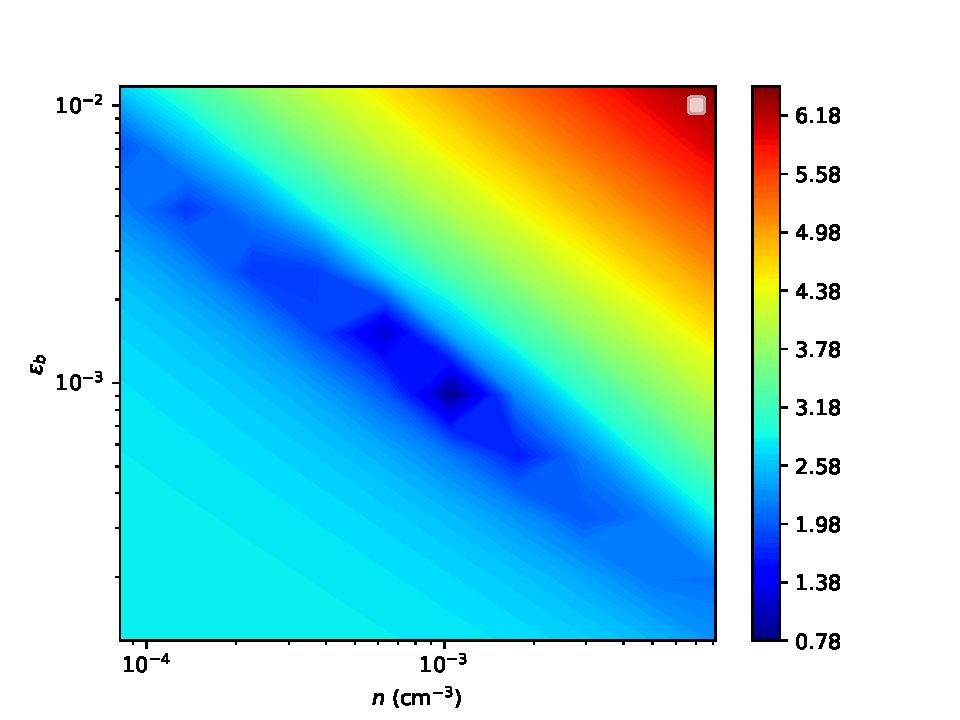
\includegraphics[width=0.48\linewidth]{n_epsilon_B}
\end{subfigure}%
\begin{subfigure}
    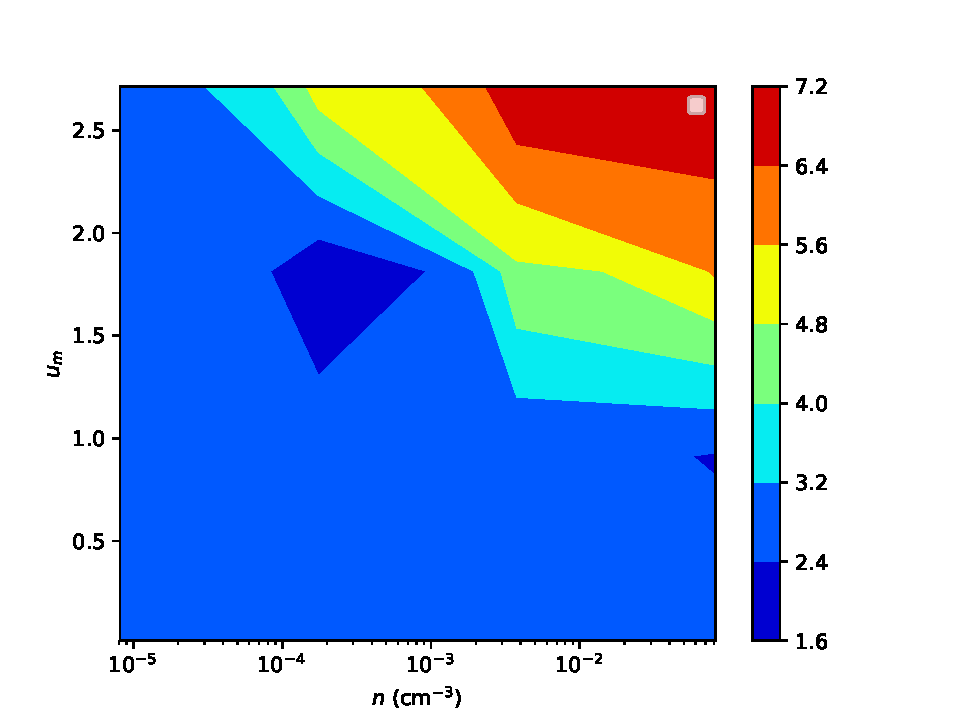
\includegraphics[width=0.48\linewidth]{umn}
\end{subfigure}
\caption[Projected likely-hood map on the fitting of the external parameters $n$ and $\epsilon_B$]{Projected likely-hood map on the fitting of the external parameters $n$ and $\epsilon_B$ (left) and $n$ and $u_m$ (right) in the radially structured ejecta model.}
\label{n_epsilon_B}
\end{figure}


Similarly, we observe a strong anti-correlation between the dynamical parameter $u_m$ and $n$, as shown Figure \ref{n_epsilon_B}. We observe that for $u_m$ values smaller than best-fit, the global fitting error is invariant long lines of constant $nu_m^{-\beta}$, where $\beta~\sim~5~=\alpha$. Coming back to the dynamical equation ($V(r) = 4\pi r^3/3$ is the volume of swept-up mass):

\begin{equation}V(r)(u_m^{-\alpha} - u_M^{-\alpha}) n c ^ 2= E_0 (u^{-\alpha} - u_M^{-\alpha}) \end{equation}

It appears that if $u_m^{-\alpha} \gg u_M^{-\alpha}$, which is the case for our $\alpha = 5$ , $u_m < \bar{u_m} \sim 1.5$ and $\bar{u_M} \sim 3.2$, then the dynamic equation simplifies to:

\begin{equation}V(r) n u_m^{-\alpha} c^2 = E_0 (u^{-\alpha} - u_M^{-\alpha}) \end{equation}

by which the dynamics are determined by the product $n u_m^{-\alpha}$ and no longer by both $n$ and $u_m$, as suggested by the anti-correlation we observe.

Also, we deduce from Table \ref{cocoon} that the best-constrained parameter is $u_m$. As explained previously, $u_m$ determines the moment when the dynamics switch from the catching-up phase to the mono-kinetic regime, consistently producing a sharp break in the dynamical behavior and thus in the light-curve. As the radio data point out, the flux features a sharp light curve maximum, and it is thus understood that the time of dynamical regime shift must be well determined and thus $u_m$ tightly constrained.\\

\bf{What \it{is} the ejected matter? }As we have seen, the afterglow does not likely originate from a relativistic jet. It is more likely in a quasi-spherical shape, and was ejected with inhomogeneous velocities. This unfortunately does not inform us on the nature of this ejected matter, i.e its composition, the process during which, when and from where it was ejected.

It is likely that the answers to these interrogations lie in the signatures of earlier phases of the phenomenon. In particular, as illustrated in Figure \ref{gbmax} and Table \ref{cocoon}, the maximum ejection velocity $u_M$ is the most poorly constrained parameter of the radially-structured quasi-spherical model, for lack of early radio points.

\fig{gbmax}{0.7}{Radially structured model light curves with varying $u_M$ and best-fit values for all other parameters. $u_M$ would be better constrained with earlier flux measurements.}{Radially structured model light curves with varying $u_M$ and best-fit values for all other parameters}

Measuring radio fluxes at earlier times would allow better constraints on $u_M$ and thus a better understanding of the ejection conditions, and therefore of the nature of the ejected matter. This of course requires more sensitive instruments.

How much more sensitive? The first measured radio points have fluxes of 17~$\mu$Jy, indicative of the limit sensitivity of current instruments. With the temporal indices of the increasing and decreasing phases of the light curve, we may infer that radio points at 10 days post merger would have required a sensitivity a factor of 1.5 better, and points at 1 day post-merger a factor of 8 better. With the current sensitivity, the radio afterglow signal should be lost at 2 years post-merger. Counting on a factor of 5 sensitivity increase with respect to current instruments announced for SKA1-mid \citep{62}, radio points would have been measured at 2 days post-merger, and the signal would continue to be followed until 7 years post merger.

All of these perspectives are promising for the study the phenomenon at earlier stages, and thus --~among other things~-- better constraints on the nature of the ejecta. Moreover, as indicated on figure \ref{n_vary}, the amplitude of the flux is correlated to the density of the external medium. Thus, denser circum-merger mediums will also render the earlier stages of the phenomenon easier to study.

Furthermore, it is possible that the matter currently plowing the exterior medium was not ejected simultaneously. Indeed, in the so-called \it{cocoon model} \citep{42, 5}, a relativistic jet impacts some previously ejected matter, depositing supplementary kinetic energy, and thereby \it{choking} the GRB. This results in no classical jet-produced GRB, but rather in a higher-energy quasi-spherical ejecta producing a weak GRB and eventually a quasi-spherical remnant and shock. Nonetheless, these models concern the origin of the shock-forming matter while our calculations are only concerned with the geometry of this matter and it's final velocity distribution.


\subsection{The external medium}
The best-fit density parameter $\sim~10^{-3}~\rm{cm}^{-3}$ value is broadly consistent with typical values inside gas-rarefied early-type galaxies such as NGC4993 \citep[e.g][]{44}.

More precisely, according to recent measurements of HI fluxes at 21~cm in the host galaxy of MMT170817 \citep{12}, an upper limit on the mean galactic density of atomic hydrogen is found to be $n_{\rm{HI}}~<~4~\times~10^{-2}~\rm{cm}^{-3}$. If we suppose that the local medium is composed essentially of hydrogen, this upper limit is consistent with our model's predictions.

Similarly, with a star formation rate measured to $\sim~10^{-2}~\Ms/\rm{yr}$ \citep{9} and using the Kennicut-Schmidt law  \citep{43}, the average density of HI in NGC4993 is estimated to $\sim~4 \times 10^{-3}~\rm{cm}^{-3}$ \citep{12}, assuming the HI content to extend out to $\sim~18~\rm{kpc}$ from the center of NGC4993. This is roughly a factor of 5 above our prediction. As illustrated in Figure \ref{galac}, the projected position of the coalescence site is well inside the bulge of NGC4993. The angular distance from the merger site to the center of the galaxy is $\sim~10.6''$, equivalent to 2.12~kpc at 40~Mpc.

Consequently, the discrepancy --~if it is significant, no uncertainties are mentioned in \citet{12}~-- in estimates of local density can be explained either by the fact that \textit{(i)} the merger site is in fact in a peripheral region of the galaxy, where the density is lower than the average, or on the contrary that \textit{(ii)} the merger site is well inside the galaxy as suggested by the projected position, but the gas and dust content of NGC4993 does not follow an ordinary radially-decreasing profile. This last possibility is further supported by the presence of shell structures in NGC4993 as shown by \citet{33}, indicating a recent galactic merger event implicating the host galaxy, therefore explaining a non-trivial distribution of gas in NGC4993 and finally the possibility for lower-than-average densities even in central regions of the galaxy.

How likely is the merger site to be in the central region of NGC4993? Supposing that the merger site was drawn from a uniform distribution of points in the galaxy of radius $R_G$, the observation of the projected radial distance at $R_\rm{proj} = 2.12$~kpc implies a posterior probability distribution for the actual radial distance $R$ from the galactic center to the merger locus. This distribution is illustrated in Figure \ref{prob}, where we have followed \citet{12} in taking $R_G = 9$~kpc (stellar extent).

We observe that this posterior distribution is essentially flat, and a simple integration shows that the peaked region around $R_\rm{proj}$ does not significantly increase the probability that the merger site be indeed at a distance $R_\rm{proj}$ from the center. Thus, we conclude that the projected position does not help to determine the actual position of the site in the galaxy, and a conclusion between cases \it{(i)} and \it{(ii)} described previously cannot be drawn.

What's more, our model shows that the spatial extent of the remnant now reaches scales of $\sim$~1~pc. On this scale, galactic density can well vary from the galactic average density. Thus, regardless of the position of the remnant in the galaxy conclusions on the discrepancy between HI-inferred densities and our model predictions cannot be taken.

The important point of this discussion of the circum-merger medium is that its number density is predicted to values compatible with those measured in typical early-type galaxies.
\fig{prob}{0.7}{Probability density distribution for the radial distance of the merger locus to the galactic center, knowing the projected radial distance to be 2.12~kpc, and supposing the merger point drawn at random in the 9~kpc-radius galaxy.}{Probability density distribution for the radial distance of the merger locus to the galactic center}


\fig{galac}{0.8}{\it{Left:} Localization of the merger site as projected on the sky plane in NGC4993. \it{Right:} Best-fit Sersic profile subtracted image of the NGC4993. Notice the shells indicating a recent galactic merger event supporting a non-trivial density profile \citep{33}.}{Localization of the merger site as projected on the sky plane in NGC4993}


\fig{n_vary}{0.7}{Radially structured model light curves with varying exterior density $n$ and best-fit values for other parameters.}


\subsection{What of the standard relativistic jet?}

We found in the previous section that the radio observations could not be understood as the afterglow emission from a jet-structured outflow. Nonetheless, in the merger event a short GRB occurred, and the standard understanding of GRBs is that they are produced by jet-structured outflows. The non-observation of a jet-like afterglow emission therefore constrains the characteristics of any relativistic jet which would have occurred and produced the GRB.

%Furthermore, if we require coherence of these constrained jets with sGRB observations and models, then constrains on the characteristics of the exterior medium are found.

Here, we will thus make the hypothesis that GRB170817A was produced by a jet, and answer the question: \it{What can we learn of this eventual relativistic jet from its non-observation until now?}, and \it{Given constraints on any eventual jet, what can we learn on GRB170817A?}

\bf{Hiding the jet afterglow.} How may we translate the non-observation of a jet in terms of jet afterglow time of peak and peak flux?

A first approach is to require that the jet-induced afterglow peak flux $F_j^p$ be weaker than the observed radio flux \it{at the time of the jet afterglow peak} $t_j^p$. This of course is a weaker constraint than to require that the jet afterglow flux be \it{weaker than the observed fluxes at all times}. We call this the \it{jet hiding} condition. A mathematical formulation is:

\begin{equation}F_j^p < F^{\rm{obs}}(\nu, t_j^p) \end{equation}

Figure \ref{fmaxtmax} illustrates our method to translate this into conditions in parameter space. Suppose that $F_j^p$ and $t_j^p$ are given in terms of a power-law on the parameters $E_j$, $n$, etc. which we will note $p_1$, $p_2$ for now. That is:

\cen{F_j^p = F_0 \,p_1^{\alpha_1} \,p_2^{\alpha_2} \dots}

and

\cen{t_j^p = t_0 \,p_1^{\beta_1} \,p_2^{\beta_2} \dots}

Then, suppose that the radio light curve be given by a power law as well, that is:

\cen{\Fobs(\nu, \tobs) = \Fobs_0 \tobs^{\gamma}}

Now, the hiding condition is thus rewritten:

\begin{equation}F_0 \,p_1^{\alpha_1} \,p_2^{\alpha_2} \dots < \Fobs_0 \,\left( t_0 \,p_1^{\beta_1} \,p_2^{\beta_2} \dots \right)^{\gamma} \end{equation}

Which in fact results in a \it{sub-linear condition} on the parameters for the jet to be hidden:

\begin{equation}(\alpha_1 - \gamma \beta_1) \log p_1 + (\alpha_2 - \gamma \beta_2) \log p_2 + \dots < \log \left( \frac{\Fobs t_0 ^\gamma}{F_0} \right) \end{equation}

The geometrical interpretation of this is simple: the indices $\alpha_i$ and $\beta_i$ are just the coordinates of the vectors by which is displaced the maximum of the jet afterglow if the parameters are multiplied by 10. The hiding condition is then simply the condition on any linear combination of these vectors so that the jet remain hidden when displacing the maximum, hence changing the underlying parameters.

\fig{fmaxtmax}{0.7}{Illustration of the method used to obtain constraints on the relativistic jet. Changing the jet parameters will displace the maximum of the jet afterglow light curve along the vectors showed here. Requiring that the maximum be always weaker than the radio points amounts to sub-linear conditions on the jet parameters.}{Illustration of the method used to obtain constraints on the relativistic jet}


After a thorough exploration of the parameter space, we infer that the peak time and peak flux of a jet-induced afterglow consistently scale like the following with the jet parameters and exterior medium parameters\footnote{The initial Lorentz factor of the ejecta $\Gamma_0$ is not relevant here because as detailed in \it{Appendix B}, the dynamics in the relativistic deceleration phase (during which the peak occurs) no longer depend on $\Gamma_0$}:

\begin{align}\label{ft}
    F_j^p &= 121~\mu\rm{Jy} \left(\frac{E_j}{10^{52}~\rm{erg}} \right)^{} \left(\frac{n}{10^{-3}~\rm{cm}^{-3}} \right)^{4/5} \left(\frac{\epsilon_B}{10^{-3}} \right)^{4/5} \left(\frac{\theta_{\rm{obs}}}{0.25~\rm{rd}} \right)^{-4.3} \left(\frac{\theta_j}{0.1~\rm{rd}} \right)^{2} \\
t_j^p &= 37.4~\rm{d} \left(\frac{E_j}{10^{52}~\rm{erg}} \right)^{1/3} \left(\frac{n}{10^{-3}~\rm{cm}^{-3}} \right)^{-1/3} \left(\frac{\theta_{\rm{obs}}}{0.25~\rm{rd}} \right)^{8/3}
\end{align}

We note that an analytical derivation of these scalings would greatly enlighten the discussion we are having here, and is part of the activity which will follow this work.

We model the observed light curve as a broken power-law as illustrated in Figure \ref{fmaxtmax}. We obtain the following:

\[
\Fobs({3~\rm{GHz}}) = \left\{ \begin{array}{lr}
							(77.6 \pm 12.1)~\mu\rm{Jy} \left(\frac{t_{\rm{obs}}}{100~\rm{d}}\right)^{0.791 \pm 0.152} & \text{if}~t_{\rm{obs}} < 163~\rm{d} \\
							(45.4 \pm 41.7)~\mu\rm{Jy} \left(\frac{t_{\rm{obs}}}{300~\rm{d}}\right)^{-1.29 \pm 1.56} & \text{if}~163~\rm{d} < t_{\rm{obs}}
							\end{array}\]

In conclusion, a set of jet parameters and exterior medium parameters will give rise to a hidden jet if:

\[ \left\{ \begin{array}{l}
			F_j^p < 77.6 ~\mu\rm{Jy} \left(\frac{t_j^p}{100~\rm{d}}\right)^{0.791} \\
			\rm{and}\\
			F_j^p < 45.4 ~\mu\rm{Jy} \left(\frac{t_j^p}{300~\rm{d}}\right)^{-1.29}
			\end{array}
\]

taking the central values on the power-law fitting of the light curve.

In turn, this translates in parameter space to\footnote{We introduce the notations $\xx{E_j} = \log \left(\frac{E_j}{10^{52}~\rm{erg}} \right)$, $\xx{n} = \log \left(\frac{n}{10^{-3}~\rm{cm}^{-3}} \right)$, $\xx{\epsilon_B} = \log \left(\frac{\epsilon_B}{10^{-3}} \right)$, $\xx{\theta_{\rm{obs}}} = \log \left(\frac{\theta_{\rm{obs}}}{0.25~\rm{rd}} \right)$, $\xx{\theta_j} = \log \left(\frac{\theta_j}{0.1~\rm{rd}} \right)$.}:

\begin{equation}
    \label{sublin}
 \left\{ \begin{array}{l}
			0.736 \xx{E_j} + 1.06\xx{n} + \xx{\epsilon_B} - 5.35\xx{\theta_{\rm{obs}}} + 2\xx{\theta_j} < -0.531\\
			\rm{and}\\
			1.43 \xx{E_j} + 0.37\xx{n} + \xx{\epsilon_B} - 0.49\xx{\theta_{\rm{obs}}} + 2\xx{\theta_j} < 0.74
			\end{array}
\end{equation}

These are two sub-linear conditions in the 5-dimensional space of jet and medium parameters which are implied by the non-observation of a jet-induced afterglow.

We will now further discuss the eventuality of a relativistic jet by specifying some values for some of the parameters in these two sub-linear conditions. These values will come from our previous results (on $n$ and $\epsilon_B$, coming from the fitting to the radially structured remnant light curve), and results from the gravitational wave signal(on $\theta_{\rm{obs}}$ mainly).

\bf{Discussion on the intrinsic characteristics of the jet.} We turn to constraining the intrinsic characteristics of the jet. Recall that we are in the hypothesis where GRB170817A was produced by a jet, and we would like to constrain this jet by its non-observation in the afterglow of MMT170817, and then constrain the GRB using the constraints on the jet.

The two sub-linear conditions in Eq.~\ref{sublin} that we have established imply all 5 parameters of a jet afterglow. If we seek constraints on the jet parameters only ($E_j$, $\theta_j$), independently of exterior factors, then we must fix the three parameters $n$, $\epsilon_B$ and $\thetaobs$. Luckily, we have estimates for $n$, $\epsilon_B$ as provided by our fitting to the radially structured model which we can take. Also, we can vary $\thetaobs$ in the range indicated by the gravitational wave data from GW170817.

Before we proceed, it is interesting to establish a scale for $E_j$ (kinetic energy of the jet outflow) which will relate the energy scale of GRB170817A and short GRBs in general.

The fluence of GRB170817A was $(2.8\pm0.2)\times10^{-7}$~erg~cm\sp{--2} \citep{52}, and the isotropic equivalent dissipated energy is thus $E^{\rm{iso}}_\gamma~\sim~5.4 \times 10^{46}$~erg. In the standard vision where the GRB was produced by a relativistic jet, this is the total kinetic energy of the pre-GRB jet which was dissipated in gamma rays. The kinetic energy of the post-GRB jet (producing the afterglow) is thus the remainder of this kinetic energy, after dissipation in radiation. By denoting $E^K_0$ the initial kinetic energy of the pre-GRB jet, we thus have:

\begin{equation}E^K_0 = E^{\rm{iso}}_\gamma + E_j\end{equation}

$E_j$ still designating the kinetic energy available for the afterglow of the jet (and which is considered by our model). We now introduce the \it{gamma efficiency} parameter $f_\gamma$, which quantifies the efficiency of the dissipation of kinetic energy into gamma rays in the GRB phase, i.e $f_\gamma = E^{\rm{iso}}_\gamma/E^K_0$. The efficiencies based on kinetic energy measurements vary from some \% to many tens of \% \citep{47,48}. Using this definition, it follows that:

\begin{equation}\label{ff}
    E_j = \frac{1 - f_\gamma}{f_\gamma} E^{\rm{iso}}_\gamma
\end{equation}

Eq.~\ref{ff} will allow us to relate the constraints on the afterglow jet energy (imposed by its non-observation) to the energetics of GRB170817A.

The constraints in the ($E_j$, $\theta_j$) plane are illustrated in Figure \ref{ejthetaj}. The non-shaded region corresponds to possible hidden jets given the likely values of $n$ and $\epsilon_B$ provided by the fitting of the afterglow with a spherical radially structured remnant.

\fig{ejthetaj}{0.7}{Constraints on the intrinsic parameters of the relativistic afterglow jet, as visualized in the $(\theta_j, E_j)$ plane for various values of $\theta_{\rm{obs}}$ below $\thetaobs^{GW} = 28$~deg. Are also present indicative energy scales corresponding to different gamma efficiencies for GR170817A knowing its isotropic-equivalent energy.}{Constraints on the intrinsic parameters of the relativistic afterglow jet, as visualized in the $(\theta_j, E_j)$ plane}

We observe that only very constraining viewing angle conditions ($\thetaobs < \thetaobs^{GW}$) significantly cut the free parameter space for the jet. Even then, jets with apertures smaller than $\sim~25$~deg can have energies larger than 10\sp{50}~erg. If the viewing angle constraint is looser ($\thetaobs > \thetaobs^{GW}/2$), these jets can have energies in excess of 10\sp{52}~erg and still be hidden.

Moreover, we note that if the jet is the one which produced GRB170817A, then the gamma efficiency remains unconstrained: if we limit the jet aperture to $\sim~25$~deg, the gamma efficiency can assume any values larger than 0.1\%.

\bf{What would we have seen as on-axis observers of these hidden jets?} As testified by the power of $-4.3$ on the $\thetaobs$ term in Eq.~\ref{ft}, the maximum signal of a jet afterglow is largely suppressed by large viewing angles. Thus, some of these hidden jets (the afterglow of which is unobserved if seen off-axis) would likely have produced important afterglows if seen on-axis.

To study this, we take a typical hidden jet (one in the white region of Figure \ref{ejthetaj}), and plot the light-curve which would have been observed with smaller viewing angles. This is represented on Figure \ref{jet_theta}.

\fig{jet_theta}{0.7}{Afterglow light curves of on-axis observers for a hidden jet ($E_0 = 10^{53}$~erg). Observe the jet-break in the jet light curves which radically change the slopes.}{Afterglow light curves of on-axis observers for a hidden jet ($E_0 = 10^{53}$~erg)}

We observe that this jet, which remains hidden for viewing angles down to $\sim~12$~deg, would have completely dominated the afterglow had it been observed with viewing angles less than $\sim~10$~deg.


\bf{Jet-induced light curve rebrightnings.} Of course, our hiding condition on the maximum of the jet afterglow does not fully characterize the non-observation of a jet afterglow. Indeed, if the jet afterglow decays slower than the $t^{-1.3}$ of the radio data, than the jet can produce a \it{rebrightning} of the light curve --~a so-called \it{bump}~--, as illustrated in Figure \ref{bump}. Thus, the parameter space which we have excluded here is in fact too loose of a constraint on the jet. In the data of MMT170817 a bump has yet to be found. At the current rate of decrease of the light curve, we predict that the afterglow will remain observable until 2 years post-merger, thus the observational constraint on an eventual jet has yet to be completed.

\fig{bump}{0.7}{A jet afterglow which complies to our hiding condition (the maximum is weaker than the data at the time of maximum), yet the afterglow is clearly apparent.}{A jet afterglow which complies to our hiding condition, yet the afterglow is clearly apparent}


\subsection{Conclusion: what have we learned?}

In studying of the 3~GHz radio fluxes from the afterglow of MMT170817, we have found that among the geometrical configurations we have explored for the outflow responsible for the afterglow of MMT170817, the one that is the most consistent with the data is  quasi-spherical. Building on this result, we have learned the following:

\begin{enumerate}
    \item A near-spherical shock was formed upon contact of ejecta with a total kinetic energy of $\sim$~10\sp{50}~erg on the circum-merger medium. The shock was first formed by matter with a Lorentz factor of $\sim$~3, and was then progressively caught-up by a tail of ejecta with Lorentz factors down to $\sim$~2, continuously injecting energy into the shock. This catching-up phase led to the slow increase of the radio synchrotron emission. The end of the catching-up phase marked the maximum of the light curve, and the beginning of a phase in which the shock is a single-speed shell.

    \item The remnant is expanding in a medium of number density $\sim$~10\sp{--3}~cm\sp{--3}, consistent with the expected densities of spheroidal galaxies such as NGC4993. Some measurements of HI densities using 21 cm fluxes indicate a global galactic mean density higher than this, implying that the merger occurred in a peripheral region of NGC4993. Nonetheless, the sky-plane-projected position found near the galactic center does not inform us more on the actual radial position of the merger point in the galaxy. Finally, NGC4993 having recently ($\lesssim$~250~Myr) taken part in a galactic merger, density variations of this amplitude on scales of the remnant's size ($\sim$~1 pc) are not excluded.

    \item If a relativistic jet was produced during the merger phenomenon, it is poorly constrained by the non-observation of its signature in the afterglow flux. More precisely, given the characteristics of the external medium deduced from the study of the remnant's geometry and dynamical structure, jets with energies in excess of 10\sp{52}~erg and opening angle smaller than 25~deg could still have escaped observation in the afterglow.

    \item This energy limit is fairly high, and relating it to the remaining kinetic energy of a post-GRB jet does not constrain the gamma-efficiency of GRB170817A, which can assume any values larger than 0.1\%. Nonetheless, even these hidden jets would have dominated the afterglow had they been seen on-axis, which should be the case for some future events, and these will likely better inform us on the role of jets in binary neutron mergers
\end{enumerate}
%\end{multicols}
